%\begin{savequote}[8cm]
%\textlatin{Neque porro quisquam est qui dolorem ipsum quia dolor sit amet, consectetur, adipisci velit...}

%There is no one who loves pain itself, who seeks after it and wants to have it, simply because it is pain...
  %\qauthor{--- Cicero's \textit{de Finibus Bonorum et Malorum}}
%\end{savequote}

%\minitoc

\chapter{Ion Trap Apparatus}
% Main points:
    % Give a working overview of the apparatus.
    % The desired audience here is 
        %   i) Future members of FastGates, 
        %  ii) Anyone building a similar experiment, 
        % iii) Readers of other chapters who want technical detail of the apparatus.
% Pre reqs:
    % Motivation for why we want this apparatus!

    A vast effort is spent on the initial build-up of the an ion trap system, but
    throughout the life of the experiment, a greater effort is spent on its daily
    maintenance.  I hope that this chapter will serve as a resource for future
    members of the FastGates team, as well as provide a useful recipe for anyone
    building a similar system. \\

    Due to the size and complexity of the system, we introduce an inital overview of
    the design, motivated by the desired functions.  As the name suggests, an ion
    trap experiment aims to confine arrays of single ions, this is achieved by
    static and dynamic electric fields which, due to the ions possesing non-zero
    electric charge, can provide trapping potentials, section~\ref{sec:The Ion
    Trap}. Due to the fragility of the internal states of the ion (these are state
    of the art sensors after all), we must take great care in isolating the ion from
    any noisy environment. This neccesitates the use of ultra-high vacuum (UHV)
    systems, section~\ref{sec:Vacuum System}, vibration isolation, and magnetic
    shielding, section~\ref{sec:Magnetic Field}. To manipulate the internal electronic states of the ion, we create
    local electric and magnetic fields using RF antennae and, in this work, lasers,
    sections~\ref{sec:Laser systems} and~\ref{sec:Narrow Line Width 729 Laser}.
    Finally, to interface with the apparatus we have built, at the time scales set by our interaction strengths, we require a sophisticated and custom control system which is discussed in section~\ref{sec:Sinara Hardware}.

\section{System Design}
\label{sec:System Design}
% Main points:
    % List of unique requirements for the system
        % Motional control
        % Single addressing
        % Standing waves
    % Solidworks models of CAD with labels
    % Block diagram of the system
    % Calcium level structure 
    % Trap package
    % High NA sandwich
    % Permanent magnets
    % MUMetal box
% Pre reqs:

    \begin{figure}[ht]
        \begin{center}
        \noindent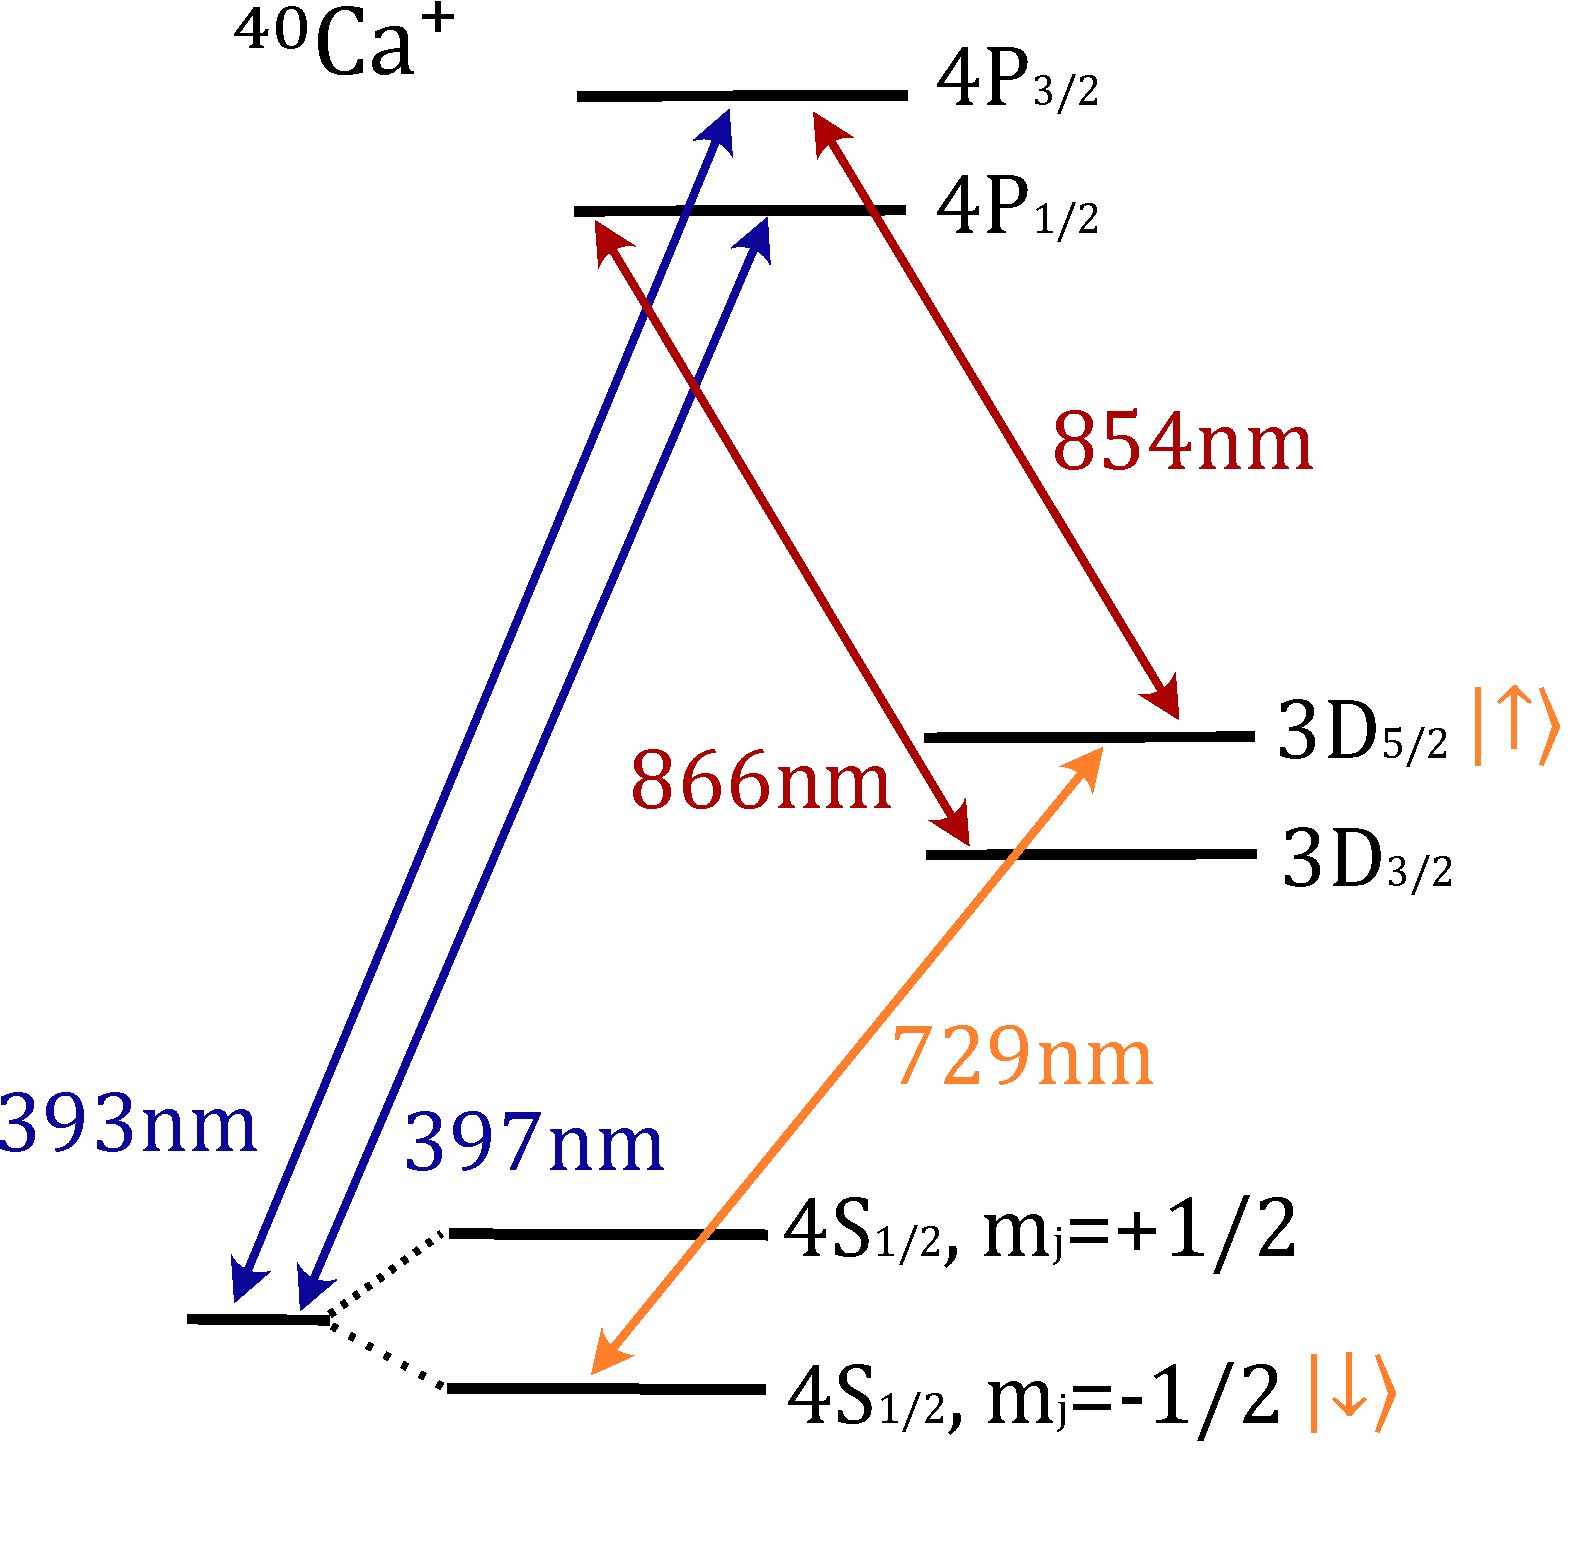
\includegraphics[width=0.4\linewidth]{figures/pdf_figure/Ca40.pdf}
        \end{center}
        \caption{
        Electronic energy levels of \textsuperscript{40}Ca\textsuperscript{+},
        which will be used in this thesis. The levels are
        split by the Zeeman effect due to a $5$~G external magnetic field (they are shown explicitely only for the ground state). The
        transitions marked are required for cooling and control over the
        ion. We shall use the optical-qubit with a quadrupole transition at
        729-nm. XXX TODO: Add zeeman levels for D5/2.
        }

    \label{fig:ion}
    \end{figure}

\section{The Ion Trap}
\label{sec:The Ion Trap}
% Main points:
    % Introduce the NPL trap chip and its advantages
    % Short intro into the parts of the ion trap DC/RF fields.
    % Fastino channels
    % Experimental parameters for stable trapping
    % Quote the values we use for trapping/experiment
% Pre reqs:
    % Motivation for trapping an ion!

    \begin{figure}
        \begin{center}
        \noindent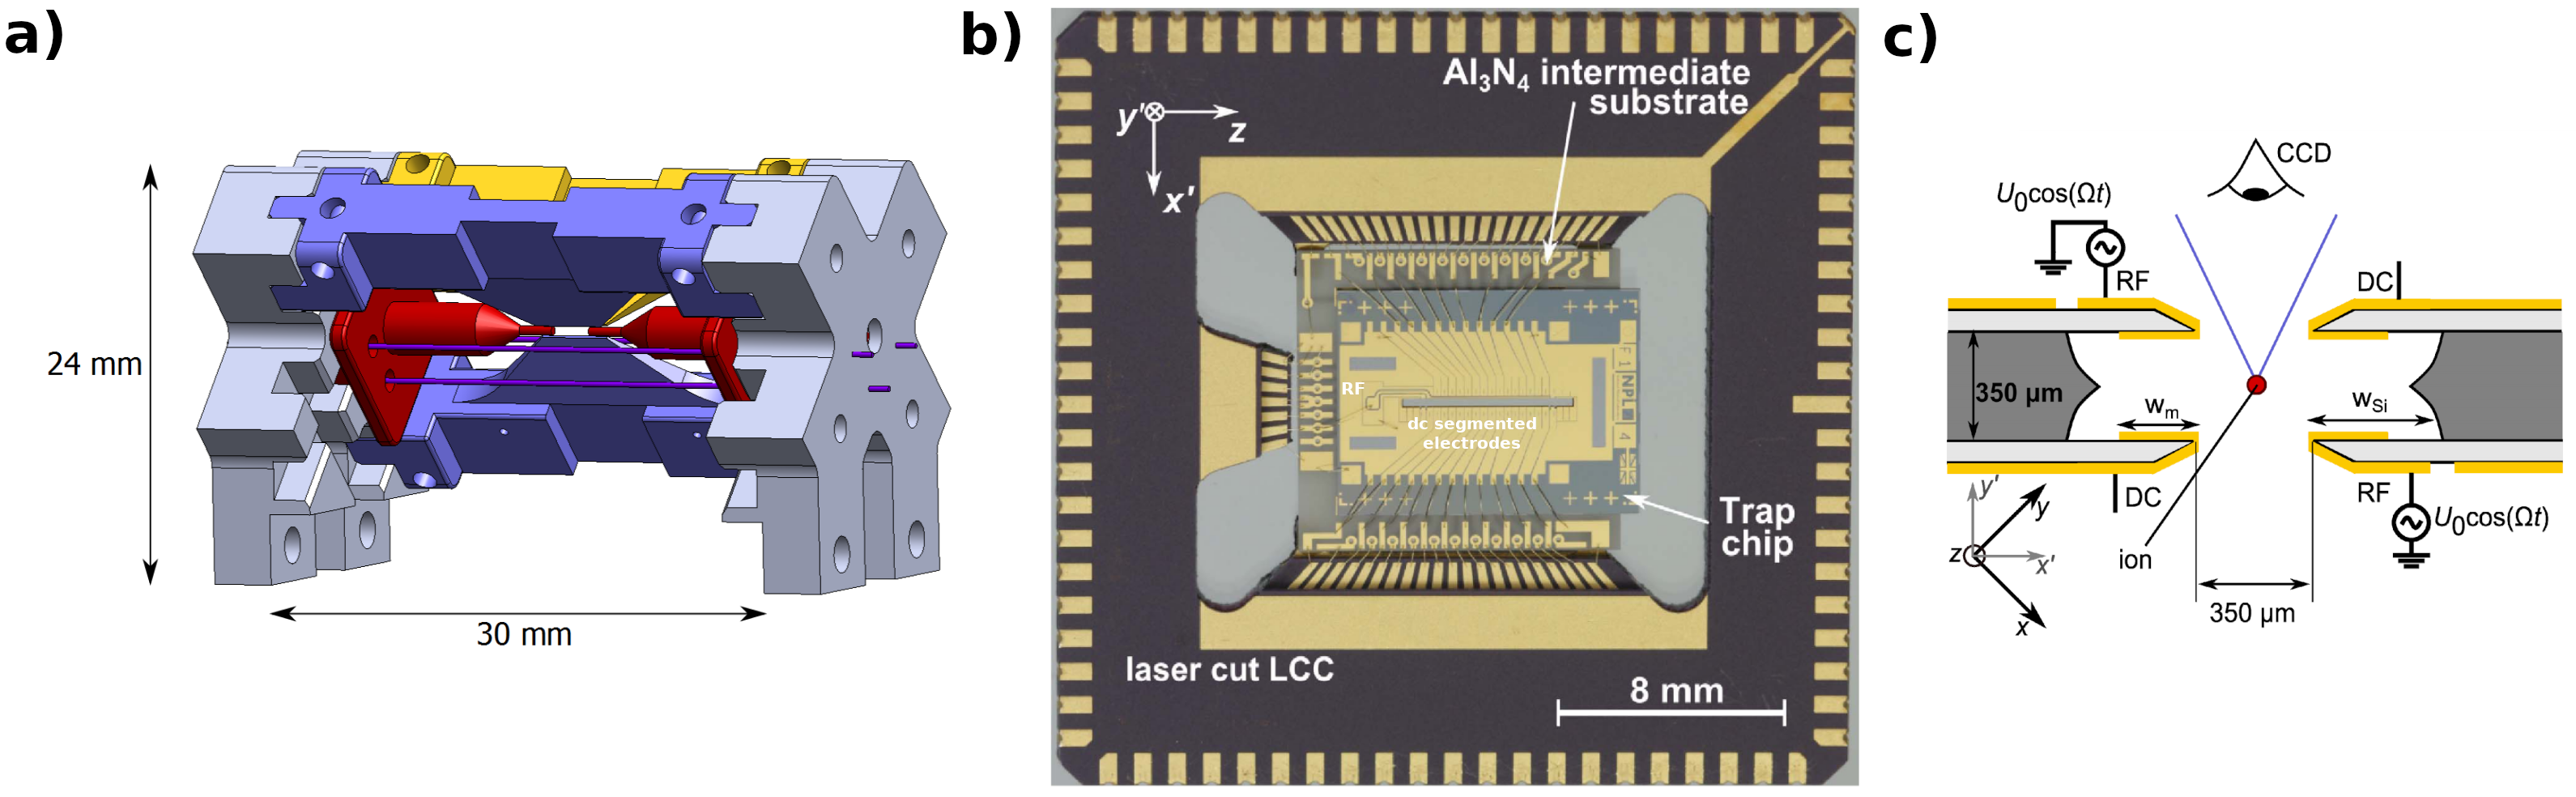
\includegraphics[width=\linewidth]{figures/png_figure/trap_comp.png}
        \end{center}
        \caption{\textbf{a)} XX Place holder figure. \textbf{b)} The NPL trap in use in this thesis. This is a microfabricated,
        segmented, multilayer trap. \textbf{c)} A cross sectional view of
        the NPL trap showing the RF and DC electrode positions.  Figures
        from~\cite{choonee_silicon_2017}.
        \label{fig:trap}}
    \end{figure}

    To create trapping potentials we use linear Paul traps, a schematic of such
    is shown in Figure~\ref{fig:trap}~(a). As explained by Earnshaw's theorem,
    $(\nabla^2 V = 0),$ a stable stationary point in 3D can not be realized
    using only static electric potentials, $V$, as if the potential is confining
    in two dimensions, it will be anticonfining in the third. Therefore, to
    achieve stable trapping either an oscillating electric field (Paul
    trap~\cite{XXX}), or a static magnetic field (Penning traps~\cite{XXX}) must
    be utilized to create a confining pseudopotential.\\
    Recently, the microfabricated surface style linear Paul trap has gained
    popularity due to the maturity of chip fabrication
    technologies~\cite{allcock_surface-electrode_2011} and the potential route
    to scalability this offers. In the surface trap, the 3D radial and axial
    electrodes of a ``macro'' trap are effectively projected onto a 2D surface.
    The stable point of such a trap is typically on the order of $50$ $\mu$m
    from the chip surface. The ease of fabrication of surface traps has allowed
    the creation of complex multizone devices with many DC electrodes.  These
    multizone traps enable the shuttling of ions, a requirement for Quantum CCD
    type architectures~\cite{kielpinski_architecture_2002}. However, this
    surface style geometry typically come with two costs: the depth of the
    trapping potential is often greatly reduced, and the close proximity of the
    surface to the ion can be a large contributor to motional heating
    rates~\cite{turchette_heating_2000}. \\
    The \emph{NPL} microfabricated 3D trap~\cite{see_fabrication_2013,
    wilpers_monolithic_2012}, as is used in our experiment, brings together the
    advantages of chip fabrication as well as the low heating rates and high
    trapping depths of a 3D style trap with greater ion-surface distances. This
    is achieved by a multilayer chip as shown in Figure~\ref{fig:trap}~(b, c).
    The radial trapping is provided by RF rails on opposite diagonals of the
    slit whilst axial trapping may be realized by the numerous DC electrodes.
    The ion-surface distance is now of the order $250$ $\mu$m and we have
    demonstrated heating rates of $ 33(3)$~q/s on a 4~MHz radial mode (see
    section~\ref{sec:Heating}).

    We aim for an axial ion separation of around $5$~$\mu$m which, for
    $^{40}$Ca$^{+}$ ions means a trapping potential of $\omega_z \approx 2\pi
    \cdot 1.6$~MHz. This ion separation was chosen to reduce the cross talk
    between ions when singly addressed (see section~\ref{sec:Single Addressing
    System}).\\ 
    We are targeting approximately $5$~MHz for our radial frequencies, as we
    shall use radial addressing for two-qubit entangling gates. The choice of
    this higher frequency is motivated by several factors. The Doppler cooling
    limit ($\overline{n} = \Gamma/\omega$, where $\Gamma$ is the transition
    linewidth and $\omega$ is the frequency of the cooled mode) inversely scales
    with the mode frequency. Consequently, higher mode frequencies result in
    lower temperatures following initial cooling. Additionally, a higher
    center-of-mass radial mode enables greater frequency separation of radial
    modes in a multi-ion crystal, which allow for greater selectivity of
    participating modes. \\ 
    Using the pseudopotential approximation~\cite{madsen_planar_2004} for the
    confining field, we can find a trapping frequency in one radial direction
    $\omega_p$
    \begin{equation}
    \omega_p = \frac{e\alpha V_{RF}}{\sqrt{2}\Omega_{RF}M\rho^2},
    \end{equation}
    where $\alpha$ is a factor of order unity given by the geometry of the trap,
    $V_{RF}$ and $\Omega_{RF}$ are the voltage and frequency provided to the
    RF-electrode, $M$ is the mass of the ion, and $\rho$ is the ion-RF electrode
    separation.  Applying some DC voltage on the axial electrodes leads to axial
    confinement with frequency $\omega_{ax}$, but must defocus the radial
    confinements as the total curvature of the pseudopotential must remain
    constant,
    \begin{equation}
    \omega_{rad} = \sqrt{\omega_p^2 - \omega_{ax}^2/2}.
    \end{equation}
    Due to the geometry of the DC electrodes with respect to the ion chain, the
    \emph{NPL} trap focuses one of the radial modes and defocuses the other when
    the DC electrodes are increased,
    \begin{equation}
    \omega_{rad\pm} = \sqrt{\omega_p^2 - (1\mp\beta)\omega_{ax}^2/2},
    \end{equation}
    where $\beta$ is some factor due to the geometry of this geometry. From
    simulation $\beta > 1$ for $\Omega_{RF} = 2\pi\cdot 23$~MHz and $V_{RF} =
    200$~V and so one radial mode increases with DC voltage applied and one
    decreases.

    \begin{table}[h!]
    \begin{center}
    \begin{tabular}{ c|c c c c c }
    & $V_{RF}$/V &  $V_{DC}$/V &$\Omega_{RF}$/($2\pi\cdot$MHz)& $\omega$/($2\pi\cdot$MHz)   & q \\ 
    &  &  & & $\omega_{ax}$\quad   $\omega_{rad}$ &  \\ 
    \hline
    Experiment  & 200 & -7 &  23 & 1.6 \quad 4.9 & 0.61 \\
    Loading  & 100 & -2 &  23 & 0.8 \quad 2.0 & 0.25 \\
    \end{tabular}
    \caption{ Simulated trapping parameters for both ``Experiment'' and ``Loading'' settings \textsuperscript{40}Ca\textsuperscript{+} with the NPL trap. The ``Experiment'' setting is optimized for high axial mode frequencies whilst the ``Loading'' setting maintains a lower q factor for practical loading.  \label{table:freqs}}
    \end{center}
    \end{table}

    A possible set of parameters to achieve $\omega_{ax} = 2\pi \cdot 1.6$~MHz
    and $\omega_{rad+} = 2\pi \cdot 4.9$~MHz can be seen in the ``Experiment''
    trapping in Table~\ref{table:freqs}.

    From the Mathieu equations, the areas of stability depend upon a factor
    $q$~\cite{berkeland_minimization_1998}, where
    $q=2\sqrt(2)\omega/\Omega_{RF}$.  Generally, we require $q$ to be as low
    ($q<0.3$) for convenient trapping.  To satisfy this requirement a
    ``Loading'' setting (with parameters in table~\ref{table:freqs}) may be used
    with $q = 0.25$ and then the $V_{RF}$ ramped to the ``Experiment'' trapping
    for high radial mode frequencies.

\subsection{Trap RF Chain}
\label{sec:Trap RF Chain}
% Main points:
    % Maybe a figure describing the elements within the RF chain
        % Frequency source (Urukul)
        % Resonator
        % RF rails
    % Quote values we use.
% Pre reqs:
    % NPL trap geometry

\subsection{Trap DC Voltages}
% Main points:
    % Describe Fastino DAC and the available electrodes on the NPL trap
    % Quote values we use.
% Pre reqs:
    % NPL trap geometry

\section{Beam Geometries and Vacuum System}
\label{sec:Vacuum System}
% Main points:
    % Technical drawing of beam geometries and magnetic field to ion chain.
    % Drawing of ion trap package with high NA lenses
    % Standing waves at the ion
% Pre reqs:
    % NPL trap
    % Why we have Dual high NA lenses
    % Magnetic field giving Zeeman shift

\begin{figure}
  \begin{center}
   \noindent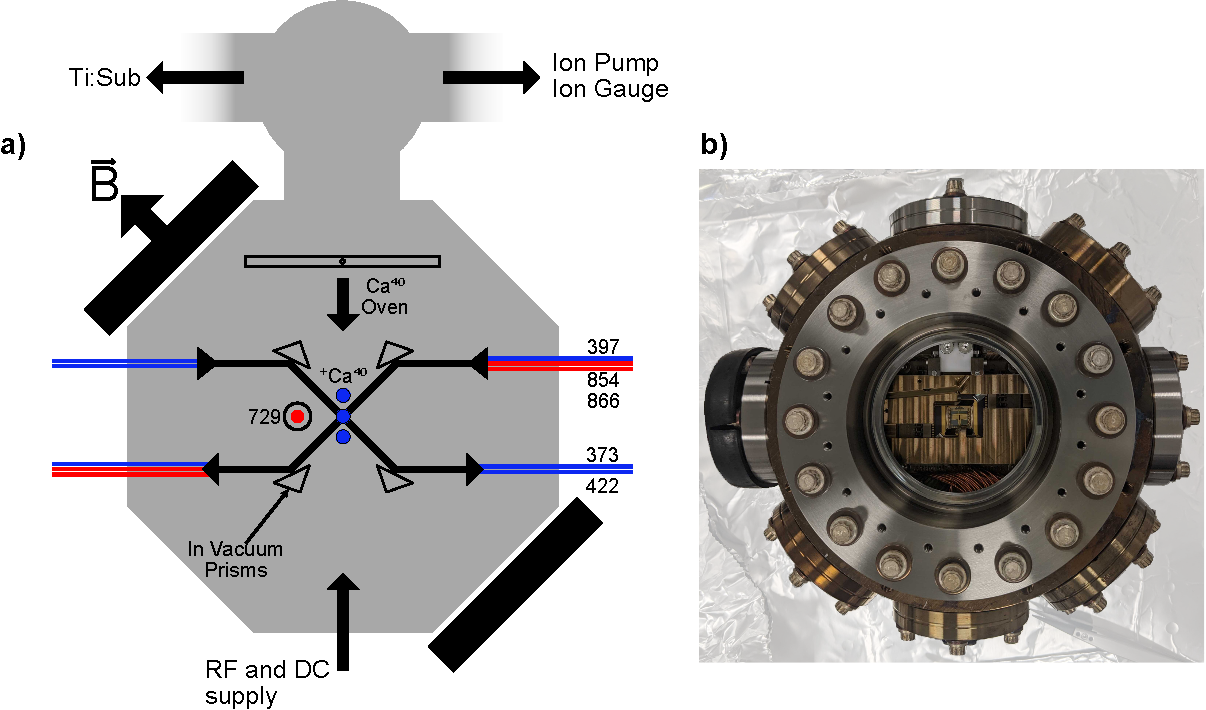
\includegraphics[width=0.9\linewidth]{figures/pdf_figure/vacuum_can-crop.pdf}
  \end{center}
  \caption{
    \textbf{a)} XXX Place holder figure. A schematic of the vacuum chamber.
    Wavelengths apart from 729-nm enter through the side CF40 viewports and are
    directed onto the ions by in vacuum prisms. The 729-nm light enters through
    the larger CF100 viewports.  \textbf{b)} A photograph of the assembled
    system prior to baking.
  }
  \label{fig:can}
\end{figure}

\subsection{Vacuum System}
% Main points:
    % List of used parts
    % What is inside the system and what is its contruction/materials
    % Operation of ion pump/Ti:Sub
% Pre reqs:

\subsection{Optical Access}
% Main points:
    % Dual High NA repeat?
    % NA for readout
    % NA for single addressing?
    % In vacuum prisms spec and design
% Pre reqs:
    % Trap package
    % Vacuum system

\begin{figure}
  \begin{center}
   \noindent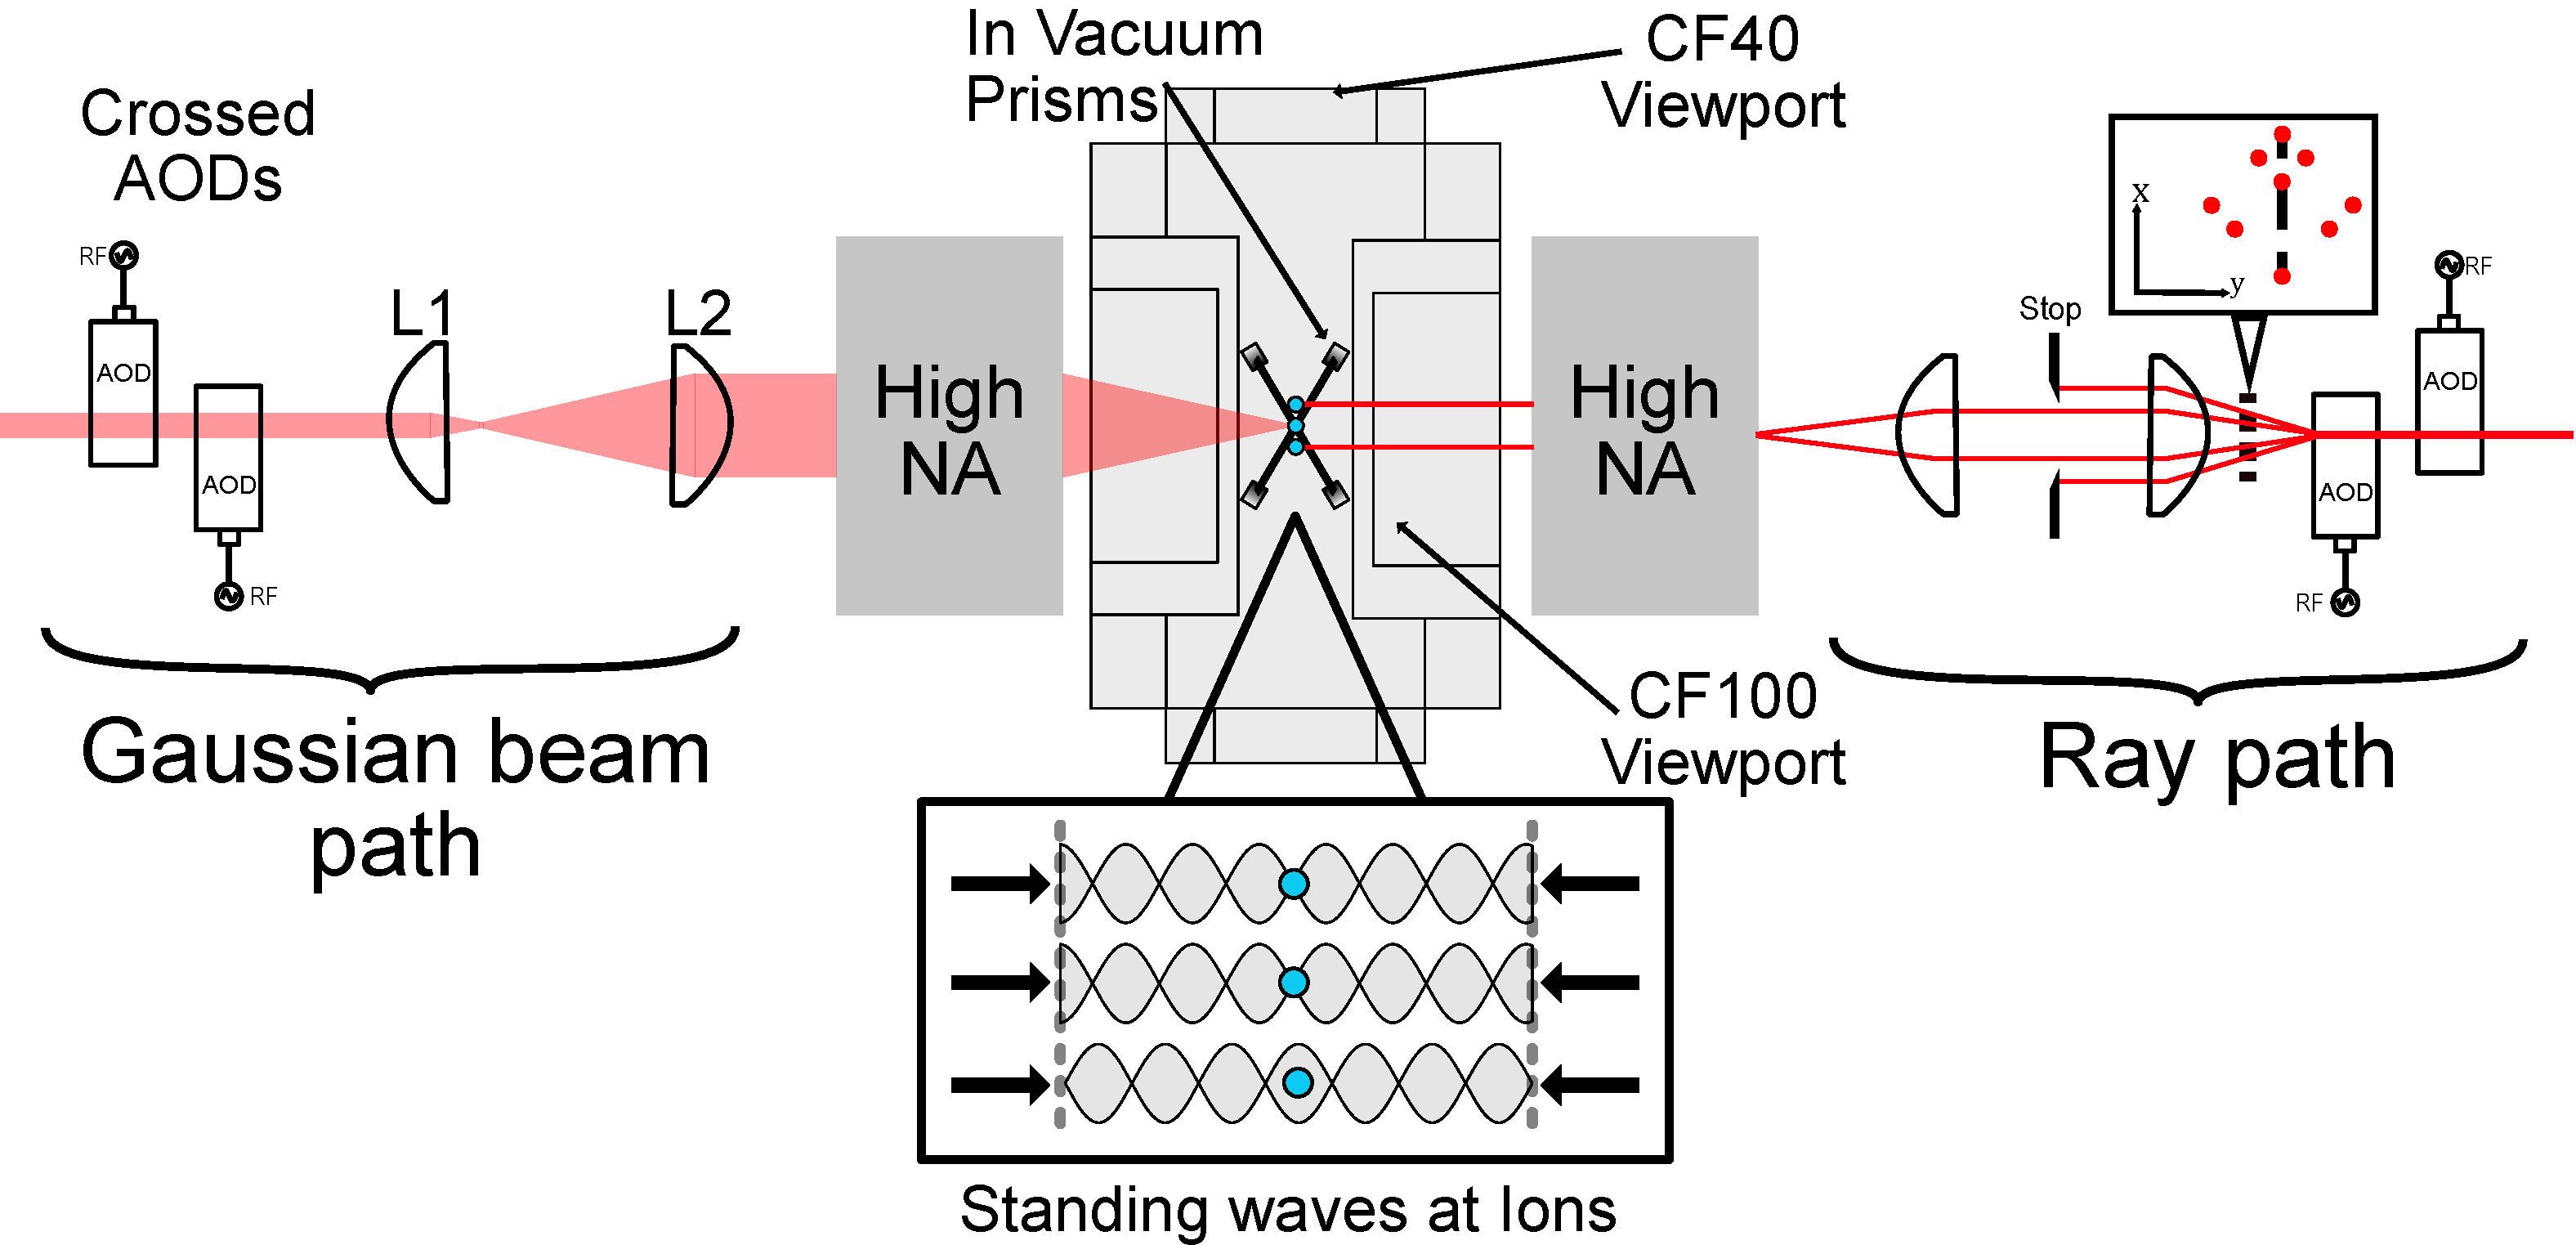
\includegraphics[width=\linewidth]{figures/pdf_figure/vac_can_AOD_small.pdf}
  \end{center}
  \caption{XXX Place holder figure. The standing wave single addressing system. Dual high NA
    objectives focus the light to a tight waist at the ions
    location. AODs are used to steer the light to only selected
    ions. The left hand side of the figure shows the Gaussian profile
    of the light, whilst the right hand side shows a ray
    representation of how two singly addressing spots are formed at
    the ions. L1 is a telecentric scanning lens and in combination
    with L2 form a beam expander.}
  \label{fig:AOD}
\end{figure}

\section{Ca$^+$ Laser Systems}	
\label{sec:Laser systems}
% Main points:
    % State which lasers we need access to
    % What frequency control do we need on each? PDH lock, AOM etc.
    % Table of all AOMs and offset frequencies
    % Table of laser powers in mW and with aimed saturation intensities for doppler idle, cooling, readout, and laser linewidths.
% Pre reqs:
    % Calcium level structure
    % 5 G field

\subsection{Narrow Line Width 729 Laser}
\label{sec:Narrow Line Width 729 Laser} 
% Main points:
    % What equipment does the 729 consist of.
    % Solstis cavity
    % Beam path and control loops (PDH, FNC)
    % Frequency shifting, pulse carving via urukul
    % Amplitude stabilisation with SUServo
% Pre reqs:
    % Calcium level structure

    Lasers are a key tool for creating the highly localised, strong electric
    field amplitudes and gradients needed to drive both carrier and sideband
    transitions of the trapped ion.\\ As shown in Figure~\ref{fig:ion}, we will
    use two levels within the 4S\textsubscript{1/2} to 3D\textsubscript{5/2}
    manifolds to define our qubit. This is an electric quadrupole transition as
    $\Delta l = 2$.  For the Calcium ion this transition is at 729-nm, and so we
    use a near resonance 729-nm laser to implement single- and multi-qubit gates
    (sections~\ref{sec:Randomised Benchmarking} and~\ref{sec:Two-Qubit
    Entangling Gates}). We also use this transition, after Doppler cooling, for
    resolved sideband cooling to bring the motional mode close to its ground
    state (as discussed in section~\ref{sec:Cooling}).

    This transition is narrrow line width due the the long lived
    3D\textsubscript{5/2} state, and so, for power efficiency, we must use a
    narrow linewidth laser. For our ``fast entangling gates'' use case we
    require large electric-field intensities at the ion to drive sideband
    transitions, this will be discussed further in the single-addressing and
    two-qubit gate sections, but here it is sufficient to say we require >100 mW
    of light at the ion plane.  Here we describe the built system 
    consisting of a Ti:Saph laser system pumped with by an Nd:YAG 532-nm laser.\\

    We pump an \emph{M2 Solstis} Ti:Saph~\cite{XXX} with 18 W of 532-nm light
    from a \emph{Coherent Verdi-V} system~\cite{XXX} to produce around 5W of
    729-nm light.  The Ti:Saph is engineered to operate with a stable $<50$~kHz
    linewidth. Ti:Saph crystals have broadband gain profiles~\cite{XXX}, which
    is often exploited in research environments to create frequency tunable
    laser systems. We however want a narrow linewidth, single frequency laser,
    and so the \emph{Solstis} has multiple intracavity frequency selective
    elements. These consist of (in order of coarse frequency selectivity), a
    birefringent filter, a tunable Fabry-P\'erot etalon, and the surrounding
    bow-tie cavity. For stable single mode operation, the \emph{Solstis} employs
    an active ``dither" servo to lock the peak of etalon transmission to one of
    the cavity longitudinal mode. This dither consists of periodically varying
    the etalon spacing with a frequency of around 20~kHz. We must be aware of
    this dither frequency as the phase modulation leads to the creation of
    sidebands on our light which can interact with the ion causing unexpected
    errors in gates. We can observe this dither frequency (and harmonics of it)
    with our ion via composite pulse experiments, however it is currently not
    expected to be a limiting source of error in any of our desired interactions
    we study.\\
    \begin{figure}
    \begin{center}
    \noindent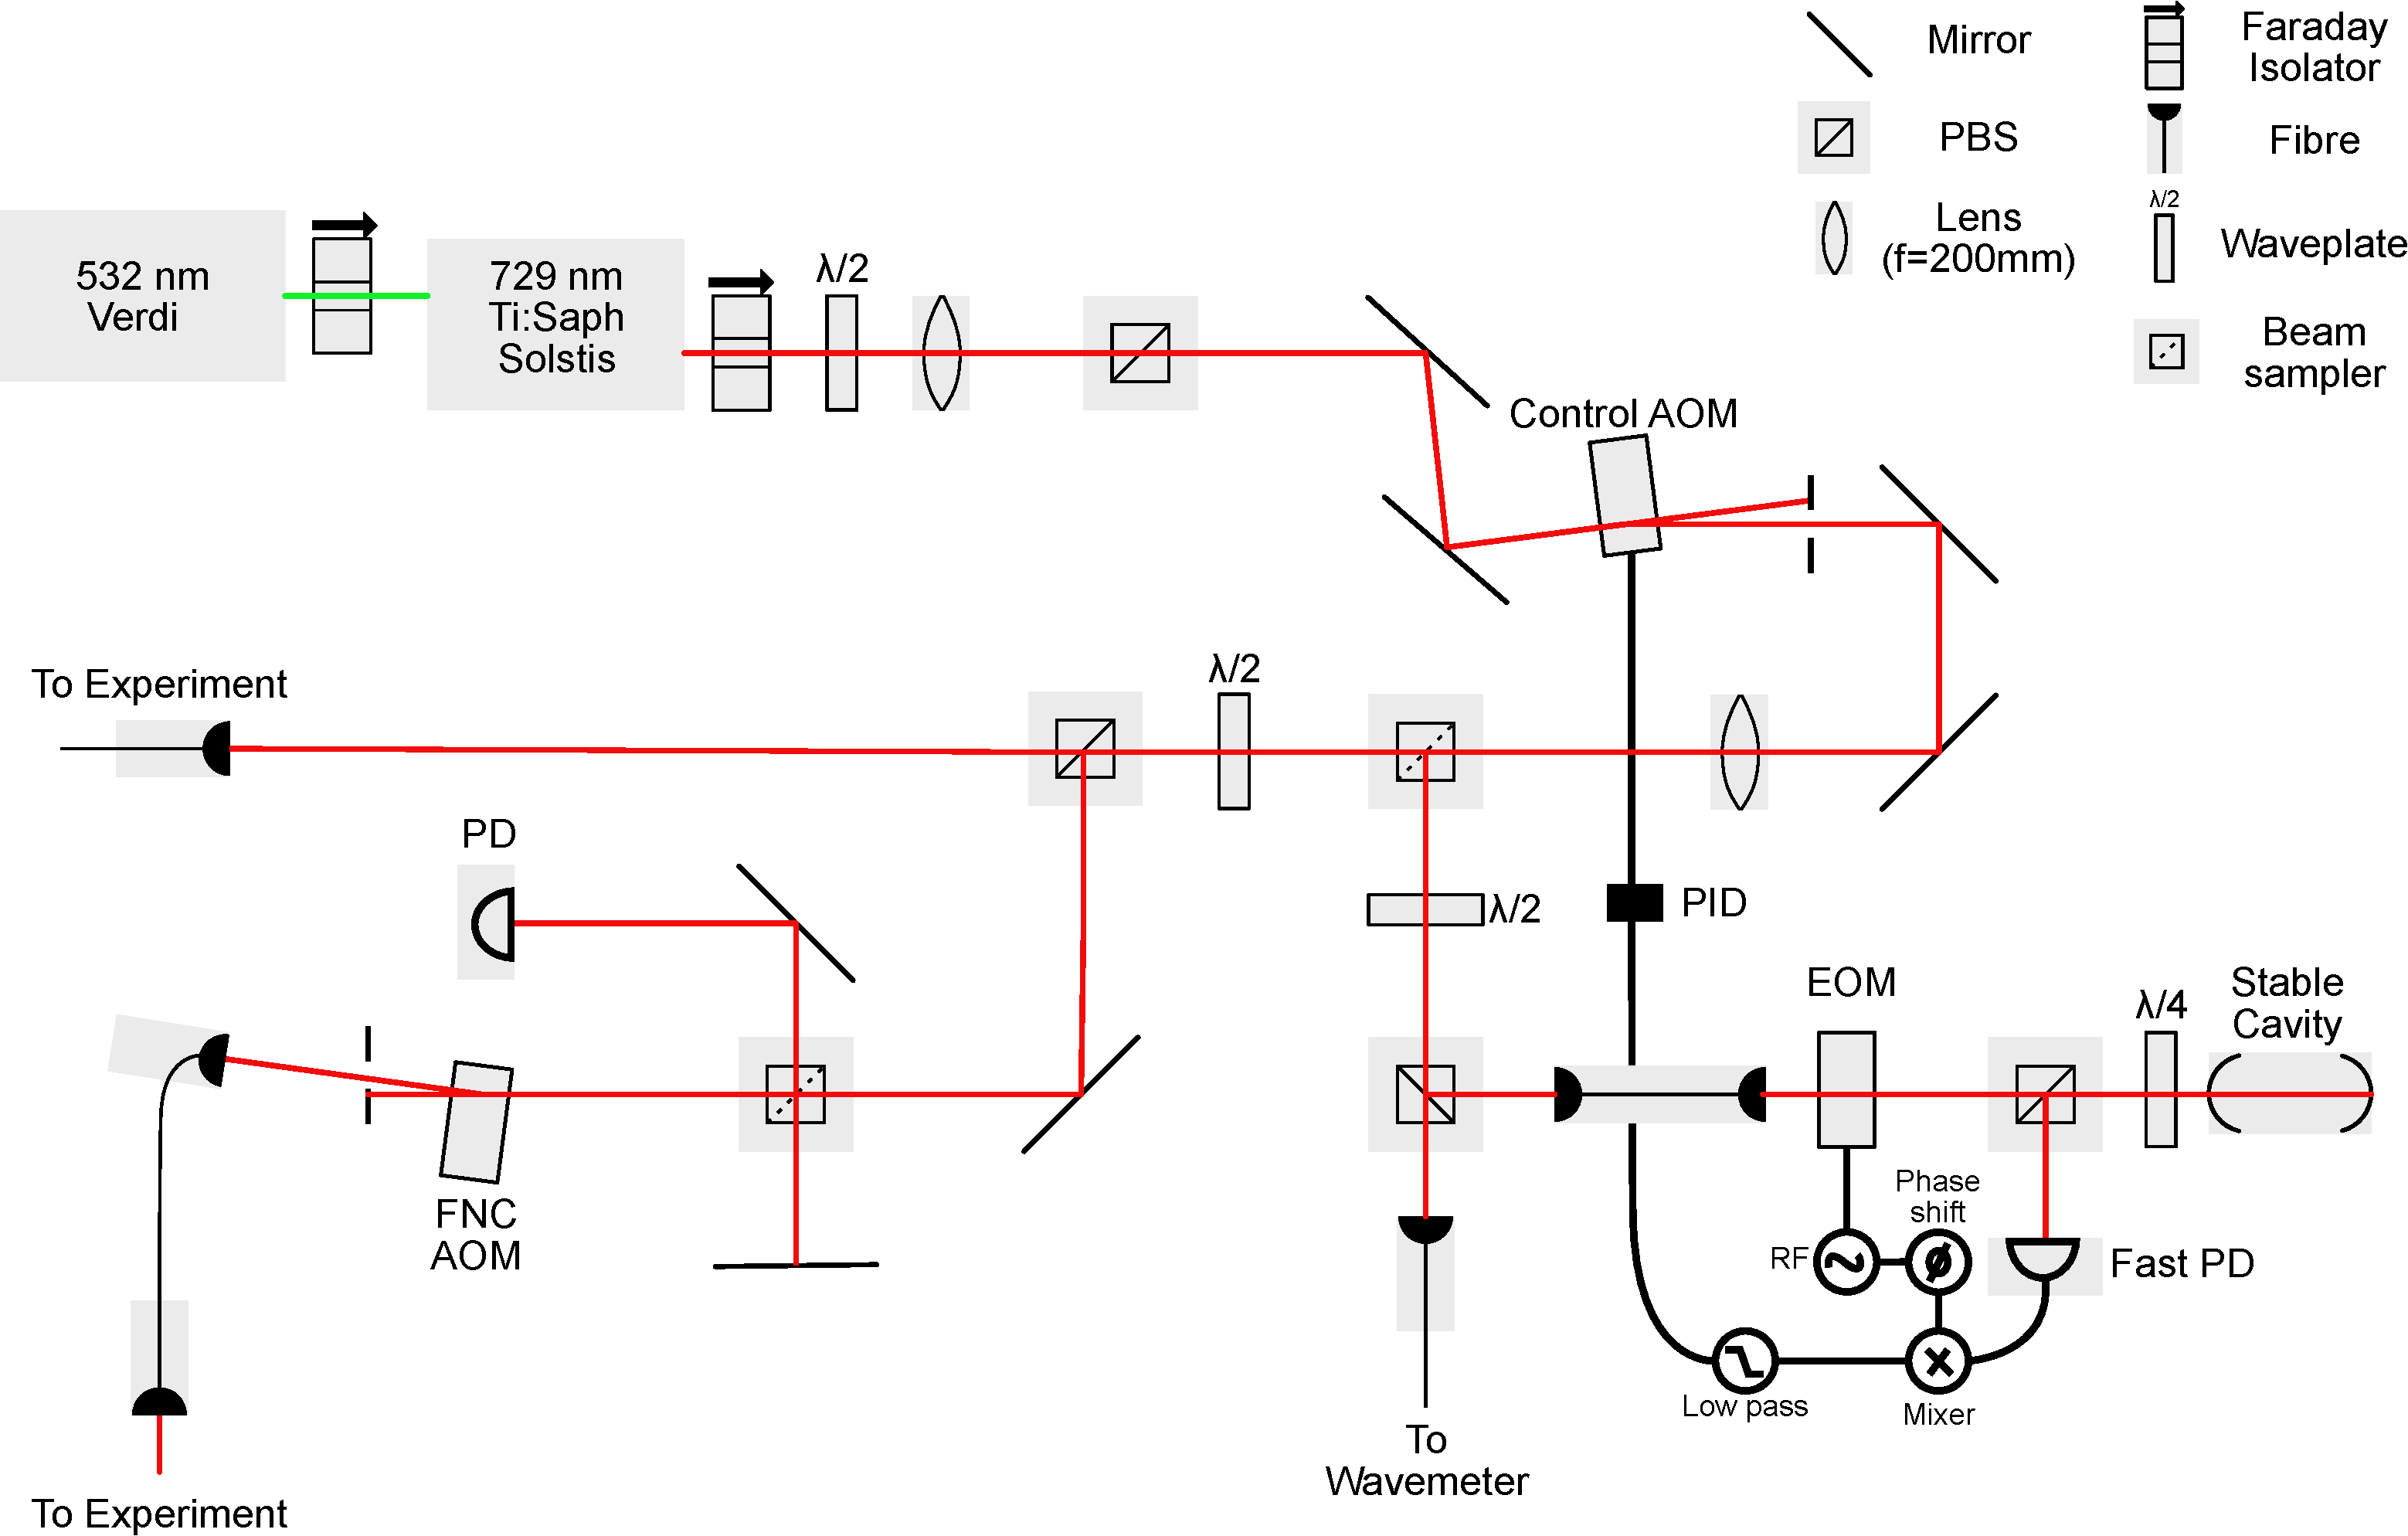
\includegraphics[width=0.9\linewidth]{figures/pdf_figure/729_path_small.pdf}
    \end{center}
    \caption{The 729-nm system. A Ti:Saph laser tuned to 729-nm is
        pumped by a 532-nm source. Light is picked off at the first beam
        sampler to stabilise by PDH locking to a cavity.}
    \label{fig:729}
    \end{figure}
    \begin{figure}
        \begin{center}
        \noindent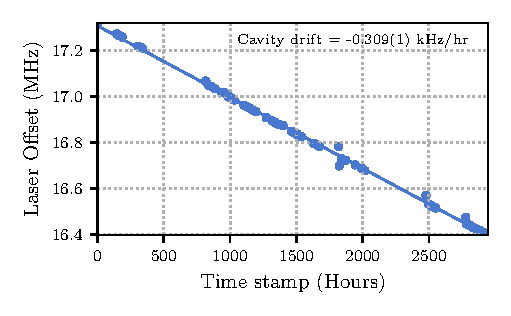
\includegraphics[width=\linewidth]{
            figures/pdf_figure/cavity_drift.pdf
            }
        \end{center}
        \caption{
            Cavity drift over 125 days. Extracted by reference to ion transition.
            }
        \label{fig:Cavity Drift}
    \end{figure}
    As mentioned, the \emph{Solstis} alone can operate with linewidths of
    $<50kHz$, however we push this further by referencing the Ti:Saph output
    with an ulta high finesse cavity by \emph{Stable Laser Systems} and applying
    a Pound-Drever-Hall (PDH) lock~\cite{}.  A schematic of our 729-nm system is
    shown in Figure~\ref{fig:729}.  PDH locking requires applying two sidebands
    via an electro-optical modulator (EOM) to the light and directing it onto
    the stable cavity. The light reflected from the cavity is then directed onto
    a fast photodetector (\emph{Thorlabs PDA10A2}). The reflection from the
    cavity consists of the interference between the carrier and the sidebands
    which have been respectively altered by the cavity transfer function. The
    photodetector signal is mixed down with the same oscillator signal as
    provided to the EOM but delayed by some chosen phase, and finally low pass
    filtered to produce a signal for use as the error signal in the servo loop.
    This error gives a measure for how far the carrier frequency is from the
    stable cavity resonant frequency and is used for feedback onto the control
    AOM situated after the Solstis. The electronics for this control loop are
    provided also by Stable Laser Systems in the form of their \emph{FPGA Servo}
    lock box. For an effective PDH lock, we require both short and long term
    stability of our reference cavity. To ensure the cavity is insensitive to
    the environment, it is made of an ultra low expansion material. We
    temperature stabilise the cavity at the zero crossing temperature of
    $30.6^\circ$C, and it is further isolated by being stored in a vacuum system
    at $<1e-7$~mbar. We measure a long term cavity drift of 309(1) Hz/hr over
    125 days, seen in figure~\ref{fig:729}. This measurement uses the ion as a
    frequency reference to probe the cavity frequency and is discussed in
    section~\ref{sec:Laser Offset}.\\
    Figure~\ref{fig:729} displays the other beam paths for our 729-nm system.
    Some light is picked off and sent to a wavemeter to continuosly monitor the
    frequency. However, the majority is coupled to two output fibres for our
    experiment and another within the group. We transport the 729-nm light from
    a dedicated laser lab to a room containing the trap apparatus by a 10~m
    single mode polarization maintaining fibre (\emph{SKXXX}).  The fibre is
    beneficial in cleaning up the mode from the Ti:Saph, however it can
    introduce phase noise due to mechanical and thermal effects along the 10~m
    length. To remove this introduced noise we utilise passive stabilisation in
    the form of thick foam tubing along the fibre length as well as active
    stabilisation by popular fibre-noise-cancellation technique~\cite{XXX}. This
    topic has been discussed extensively in multiple PhD and Masters
    theses~\cite{XXX}, and so here we only quote the relevant control aspects of
    our arrangement. We use the \emph{Sinara Stabilizer}~\cite{XXX} board, a
    dual channel PID microcontroller, with the \emph{Pounder}~\cite{XXX}
    mezzanine board, a dual channel PDH lock generator. The FNC PID software was
    developed by Ayush Agrawal ~\cite{XXX}. A comparison of spin coherence times
    is shown in section~\ref{sec:Coherence} with and without fibre noise
    cancellation enabled. \\


\subsection{Single Addressing System}
\label{sec:Single Addressing System}
% This section is not used in any characterisation - could be left for outlook!
% Main points:
    % The advantages of single addressing using AODs
        % Ion selectivity
        % High intensity electric field
    % single addressing system creating standing waves
    % render of single addressing system
% Pre reqs:
    % 729 system
    % High NA
    % Trap package
    % Motivation for future experiments